\documentclass[oneside,10pt]{swissi}

\addbibresource{4-bib/2-bib.bib}
\newcommand{\papertitle}{A regulatory-compliant AI and verification system for higher education under ESG-aligned constraints}
\newcommand{\papersubtitle}{}

\newcommand{\papercitationauthors}{Kurz, W. and Malara, M. and Stricker, W.}

\newcommand{\paperauthors}{%
  Walter Kurz\textsuperscript{1}%
  , Michel Malara\textsuperscript{1}%
  , Wojtek Stricker\textsuperscript{1}%
}

\newcommand{\paperaffiliations}{%
  \textsuperscript{1}Swissi Institute for AI,
  \href{mailto:kurz@swissi-ai.institute}{kurz@swissi-ai.institute};
  \href{mailto:malara@swissi-ai.institute}{malara@swissi-ai.institute};
  \href{mailto:stricker@swissi-ai.institute}{stricker@swissi-ai.institute}%
}

\newcommand{\paperdeclarationaffiliations}{%
  \begin{tabular}[t]{@{}l@{}}
    \textsuperscript{1}Swissi Institute for AI,
    \href{mailto:kurz@swissi-ai.institute}{kurz@swissi-ai.institute};
    \href{mailto:malara@swissi-ai.institute}{malara@swissi-ai.institute};
    \href{mailto:stricker@swissi-ai.institute}{stricker@swissi-ai.institute}%
  \end{tabular}%
}

\newcommand{\papercorresponding}{%
  Walter Kurz,
  \href{mailto:kurz@swissi-ai.institute}{kurz@swissi-ai.institute},
  \href{https://orcid.org/0009-0006-8045-4775}{ORCID 0009-0006-8045-4775}%
}

\newcommand{\paperfunding}{%
  This research received no external funding.%
}
\newcommand{\paperconflictsofinterest}{%
  The authors declare no conflicts of interest.%
}
\newcommand{\paperdataavailability}{%
  The data and code supporting this article are available from the corresponding author on reasonable request.%
}
\newcommand{\paperaitools}{%
  Generative AI tools were used for editorial work only, such as language editing and formatting, in accordance with international scientific standards. The authors verified the content and remain fully responsible for the article.%
}
\newcommand{\paperauthorcontributions}{%
  All authors contributed equally to this article.%
}

\providecommand{\swIncludeAuthorExamples}{}

\title{\papertitle \\[0.35em]
\normalsize \papersubtitle}

\author{{\fontsize{8}{10}\selectfont\paperauthors}\\[0.9em]
{\scriptsize\paperaffiliations}}
\date{\vspace{1.5em}}

\begin{document}
\maketitle

\begin{abstract}
This paper introduces a formal system model for integrating artificial intelligence and distributed verification into higher education under European regulatory constraints. The architecture consists of two interlinked components: UniAI, a role-specific, multi-agent artificial intelligence framework for institutional operations; and UniDVS, a decentralised verification infrastructure for regulatory audit, credential authentication, and tamper-evident recordkeeping. The model encodes legal instruments such as the GDPR, EU AI Act, EQF, ECTS, and ESG directives as structural system constraints, with additional compatibility for financial frameworks including MiFID II, MiCA, AMLD, DORA, and Swiss equivalents (FMIA, FinSA, FADP). UniAI agents are formalised by stakeholder class and governed by a constrained optimisation function ensuring legally admissible outputs. UniDVS operates as a DAG-based, permissionless ledger maintained by a federated educational consortium, supporting verifiable academic tokens, programmable stablecoins, and audit-ready interactions. Results are presented as a theoretical framework for compliant digital infrastructures, with direct applicability to cross-jurisdictional academic ecosystems. The model provides a foundation for regulatory prototyping, governance simulation, and controlled empirical validation.
\end{abstract}

\keywords{Regulatory technology, artificial intelligence in education, multi-agent AI systems, decentralised verification, academic tokenisation, GDPR compliance, EU AI Act, digital credential infrastructure, ESG governance, UniAI, UniDVS}

\bigskip

\section{Introduction}

The integration of artificial intelligence and distributed verification infrastructure into higher education remains fragmented and technically inconsistent. Current institutional systems lack a coherent foundation for AI-supported processes and do not enable verifiable, cross-institutional certification. This paper presents a theoretical framework for a combined architecture that integrates multi-agent artificial intelligence and distributed verification within a single, regulation-aligned system design.

The digital infrastructure of higher education has developed incrementally through proprietary software from commercial vendors. These systems address isolated administrative or instructional tasks and are rarely embedded in core institutional logic. Interoperability is limited, auditability remains weak, and institutional data structures are confined to local silos. Long-term verifiability, regulatory traceability, and technical standardisation are not structurally embedded. Artificial intelligence allows redesign of educational processes across all levels, from instructional interaction to compliance automation.

Existing systems lack the architectural capacity to support fully integrated AI operations. Most implementations are restricted to functions such as chatbots, grading tools, or plagiarism detection. These remain disconnected from assessment logic, credential management, and institutional accountability. A structured, agent-based AI architecture is required to meet the operational demands of administrators, teaching staff, students, and auditors.

\section{Related Work}

The OECD’s Collective Intelligence Model for Education (CIME) outlines a policy-based approach to integrating artificial intelligence into educational assessment. It combines psychometric modelling, large language models (LLMs), and expert oversight to support personalised feedback mechanisms \cite{okubo2025cime}. CIME provides a high-level conceptual foundation but is limited to competence diagnostics. It does not cover certification infrastructure, institutional auditability, or jurisdictional interoperability. Bernacki et al.\ conducted a systematic review of 376 empirical studies on personalised learning systems and identified a lack of conceptual convergence across implementations \cite{bernacki2021systematic}. Most systems apply adaptive logic without theoretical grounding or institutional alignment. Developer assumptions often replace pedagogical frameworks. These systems rarely include verifiability or stakeholder-specific audit capacity. Recent OECD research confirms the viability of AI scoring for large-scale international assessments using deep learning models trained on multilingual corpora \cite{okubo2023aiscoring}.

The consistency between AI-generated scores and human evaluations across psychometric dimensions shows that multilingual, AI-driven assessment functions reliably in regulated contexts. Fedus et al.\ demonstrate the feasibility of deploying trillion-parameter language models with reduced computational overhead by introducing the Switch Transformer architecture \cite{fedus2022switch}. These advances enable large-scale AI systems to operate within the resource limits of public education institutions. Sun et al.\ present ERNIE 3.0, a model that integrates structured knowledge into foundational pre-training. It improves performance across multilingual NLP tasks and surpasses human baselines on the SuperGLUE benchmark \cite{sun2021ernie3}.

The use of domain-specific knowledge is directly relevant for regulatory alignment and semantic robustness. Xue et al.\ propose mT5, a multilingual extension of the T5 model trained on 101 languages. It outperforms earlier architectures on zero-shot benchmarks and reduces translation artefacts \cite{xue2020mt5}. The model provides a foundation for AI systems that function reliably across linguistic and jurisdictional settings. Wang et al.\ introduce a zero-label learning paradigm using few-shot prompting to generate synthetic training data. Task-specific models trained this way outperform supervised baselines without relying on human annotation \cite{wang2021zerolabel}. This is suitable for institutions with limited access to high-quality labelled datasets and supports decentralised model training in federated environments. Grech and Camilleri examine blockchain-based credentialing systems such as Blockcerts and confirm the viability of tamper-evident digital diplomas \cite{grech2017blockcerts}.

These systems typically operate outside formal educational frameworks and are not integrated with European regulatory instruments such as the Bologna Process, EQF, or GDPR. Verification remains a post-hoc process rather than a native component of the educational lifecycle. Rodriguez et al.\ examine the role of artificial intelligence, blockchain, cloud computing, and data technologies (ABCD) in shaping learning assessments in higher education \cite{rodriguez2025abcd}. Their empirical study shows that institutional support and policy alignment are more decisive for adoption than technical features. The findings underscore the need for trust mechanisms and infrastructural coherence, both of which are embedded in the system model proposed here. Flanery et al.\ advocate a decentralised education framework based on Web 3.0, Decentralised Identifiers (DIDs), and blockchain-based credentialing \cite{flanery2023web3edu}.

Their proposal challenges the institutional monopoly on credential verification by enabling learners to control their own records. This aligns with the distributed verification infrastructure (DVS) introduced in this paper, particularly with respect to cross-institutional authentication, immutability, and user-controlled data architecture.

\section{Contribution}

This paper presents a unified system model that integrates multi-agent artificial intelligence with distributed verification infrastructure for higher education. Existing approaches typically focus on either pedagogical personalisation or isolated credential verification. The proposed model embeds both within a coherent, regulation-aligned architecture. It defines an AI-based institutional framework structured around stakeholder-specific agency, covering students, faculty, administrators, and auditors. Cross-jurisdictional auditability is enabled through a decentralised, tamper-resistant verification layer.

The system aligns structurally with European regulatory instruments, including the Bologna Process, the European Qualifications Framework (EQF), the European Credit Transfer and Accumulation System (ECTS), the General Data Protection Regulation (GDPR), and the EU Artificial Intelligence Act. It remains adaptable to other regulatory environments. The architecture also integrates Environmental, Social, and Governance (ESG) logic as a structural component. While ESG frameworks are not mandatory for higher education institutions, their inclusion supports macroeconomic responsibilities and prepares systems for future requirements concerning ESG ratings, whether regulatory or voluntary.

The technical design supports distributed implementation across educational institutions, coordinated by a federated consortium. This governance model prevents vendor dependency and maintains operational neutrality. The infrastructure includes tokenised academic credits and regulatory documents. These tokens represent verifiable claims on distributed ledgers and enable persistent, machine-readable certification and institutional audit.

The system also supports decentralised academic publication, network-wide peer review, and compliance-based integration of approved digital financial assets under supervisory authorities such as FINMA, BaFin, or the FMA. Combining decentralised computation with structured artificial agency, the model addresses structural gaps in educational verifiability, institutional interoperability, and regulatory traceability. It provides a theoretical foundation for future system prototyping and empirical validation.

\section{Research}

This paper conceptualises a high-level system model that integrates artificial intelligence and distributed verification into the institutional infrastructure of higher education. The model is not a technical implementation but a regulatory-aligned architectural construct. Its function is to provide a design foundation for prototyping, simulation, and empirical evaluation. The research is positioned at the intersection of computer science, educational systems design, and legal-institutional analysis. It draws methodologically on system architecture, regulatory modelling, and multi-agent design. The premise is that verifiable, scalable, and jurisdiction-compliant educational infrastructures cannot result from isolated software products or AI applications. Structural transformation requires design models that are technically coherent and legally operable across institutional boundaries.

To illustrate the proposed system at a high level, Figure~\ref{fig:UniAI-architecture} shows its layered structure across deployment, compliance, and oversight. The model separates centralised optimisation from local institutional adaptation. Each institution operates a customised instance under verified compliance and auditability.

\begin{figure}[H]
\centering
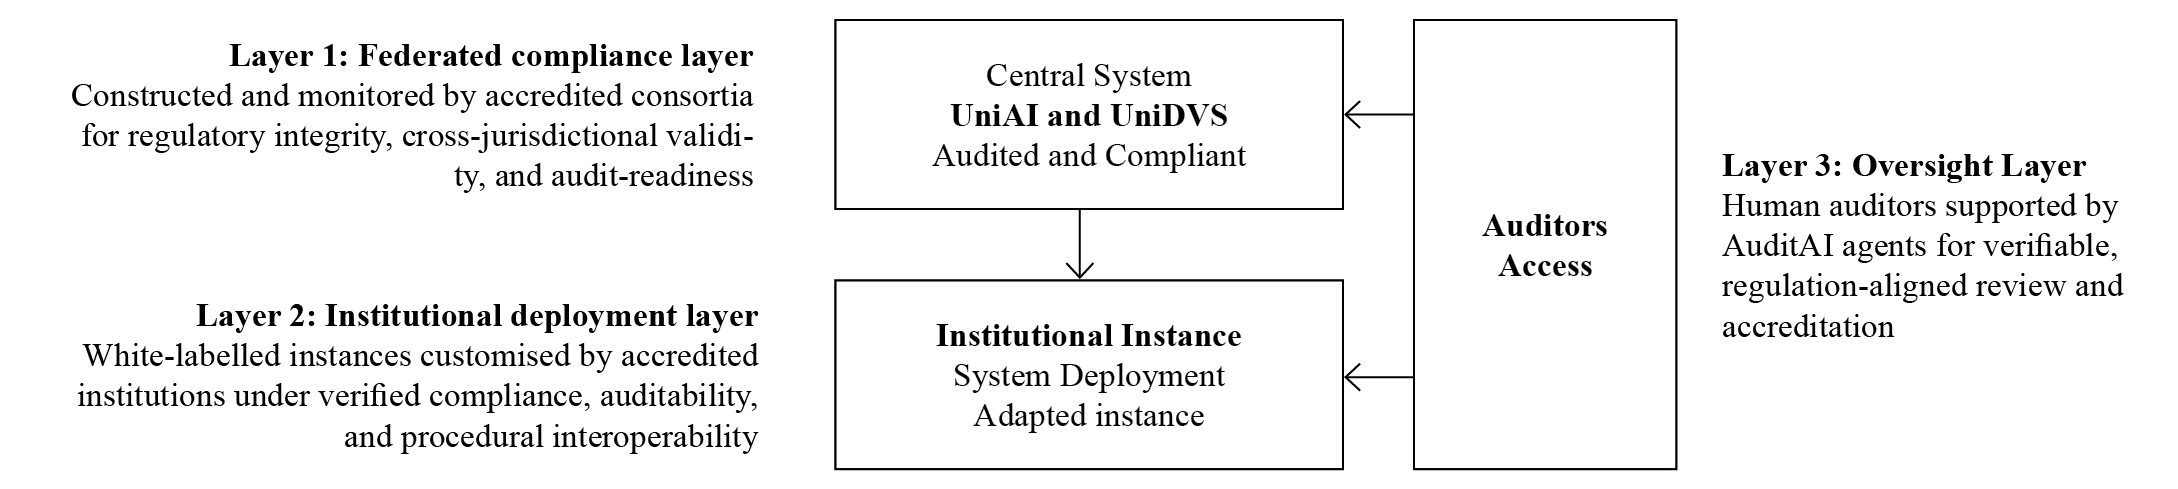
\includegraphics[width=\textwidth]{3-assets/1-User/DrWalterKurz_UniAI-1.png}
\caption{Conceptual architecture of the UniAI and UniDVS system.}
\label{fig:UniAI-architecture}
\end{figure}

Layer 1 defines the federated compliance environment managed by accredited educational consortia. The central system is trained, validated, and monitored under regulatory constraints to ensure cross-jurisdictional compliance and audit readiness. Layer 2 enables institutional deployment. Accredited institutions operate white-labelled system instances adapted to local procedures. These maintain verifiability, data integrity, and procedural conformity. Layer 3 provides oversight access for auditors and accreditation bodies. AuditAI agents support evidentiary review. Auditors assess compliance at the central layer, which includes system design, training, and constraints, and at the institutional layer, which covers programme operations, records, and credential processes.

This structure reflects the separation between system integrity and institutional flexibility. Core components are centrally governed for legal admissibility and interoperability. Institutions retain control over deployment. Independent auditors, supported by AuditAI, evaluate compliance at Layer 1 and review institutional conformity through Layer 2 outputs.

\subsection{Regulatory Context}

The system is formulated as an objective-under-constraints model. Its functional logic is guided by regulatory boundaries. Legal instruments are treated as structural constraints encoded within system design. This section examines the regulatory frameworks integrated into the operational definition of the model.

The proposed architecture operates within the regulatory landscape defined by binding and non-binding legal instruments in European higher education. The Bologna Process provides the intergovernmental framework for harmonising academic degrees, credit systems, and quality assurance across European Higher Education Area (EHEA) member states \cite{ehea2020bologna}. Its operational instruments include the European Qualifications Framework (EQF), which defines level-based learning outcomes and supports cross-jurisdictional recognition \cite{ec2017eqf}, and the European Credit Transfer and Accumulation System (ECTS), which quantifies student workload and supports credit mobility and accumulation \cite{ec2015ects}.

Personal data protection and algorithmic accountability are governed by the General Data Protection Regulation (GDPR) \cite{eu2016gdpr} and the EU Artificial Intelligence Act \cite{eu2024aiact}. GDPR requires data minimisation, purpose limitation, and transparency. These provisions apply directly to the processing of student data and algorithmic scoring in educational contexts. The Artificial Intelligence Act introduces a risk-based classification for AI applications and defines obligations concerning transparency, human oversight, and data governance. Educational and vocational training systems are explicitly included in the high-risk category.

In Switzerland, the Federal Act on Data Protection (FADP) mirrors the GDPR in its core principles and enforcement logic. It adds relevance for cross-border data flows and institutional collaboration involving Swiss entities \cite{ch2020fadp}. These frameworks define the compliance boundaries for the design of educational AI and verification systems across Europe and affiliated jurisdictions.

Accreditation requirements for institutions operating within the EQF-aligned environment are defined by the European Standards and Guidelines for Quality Assurance in the European Higher Education Area (ESG), developed by the European Association for Quality Assurance in Higher Education (ENQA) \cite{enqa2015esg}. These standards form a common basis for internal and external quality assurance. Institutions are required to implement procedures consistent with the structural logic of the Bologna Process, EQF, and ECTS.

Institutional compliance is assessed by national quality assurance agencies, which must hold ENQA membership and undergo periodic external review. Examples include the Swiss Agency of Accreditation and Quality Assurance (AAQ) \cite{aaq2024}, the German Accreditation Council through agencies such as AQAS and ACQUIN \cite{germanaccreditation2022}, the Dutch-Flemish Accreditation Organisation (NVAO) \cite{nvao2023}, and Spain’s National Agency for Quality Assessment and Accreditation (ANECA) \cite{aneca2023}. In Switzerland, the Federal Act on Funding and Coordination of the Higher Education Sector (HEdA) defines the legal basis for institutional accreditation. Formal evaluations are conducted by AAQ in accordance with ESG and international peer review principles \cite{heda2020}. Institutions not accredited under HEdA are not authorised to award legally recognised degrees or participate in state-subsidised programmes. Although Environmental, Social, and Governance (ESG) frameworks are not legally binding for higher education institutions, the model incorporates them as normative constraints. The Corporate Sustainability Reporting Directive (CSRD) and the EU Taxonomy Regulation introduce ESG principles into European regulatory instruments, especially in contexts involving public reporting, endowment management, or participation in public-private consortia \cite{eu2023csrd, eu2020taxonomy}. These instruments require transparent disclosure of environmental impact, social responsibility, and governance structures, including aspects related to digital infrastructure and institutional risk management. Recent studies show that ESG criteria increasingly intersect with AI governance \cite{lee2024esgai, perera2024esgrai}. ESG is treated not as an ethical orientation but as a structural constraint affecting system design, transparency, and institutional accountability. Key concerns include energy use in AI training and inference, mitigation of algorithmic bias, and the institutional obligation to ensure oversight, explainability, and equitable access. Embedding ESG into the model enables tracking of energy consumption, integration of fairness metrics, and creation of verifiable governance records for algorithmic outputs. Within the proposed system, ESG principles function as embedded constraints that support institutional credibility, sustainability, and operational resilience across jurisdictions. The proposed system architecture supports the issuance and verification of stable, tokenised digital assets for internal documentation, accounting, and credit transfer. These assets comprise two categories. The first includes regulated financial tokens that qualify as financial instruments under Swiss and European law. They are structured as institutionally issued stablecoins. These represent non-volatile digital units of monetary value or enforceable claims and are used to support internal transactions, contractual obligations, and service entitlements. Within the system, such tokens formalise disbursements, automate accounting, and enable programmable compliance through tamper-evident records. Deployment of these instruments requires compliance with binding financial regulation across jurisdictions. In Switzerland, applicable statutes include the Financial Market Infrastructure Act (FMIA), the Anti-Money Laundering Act (AMLA), and the Financial Services Act (FinSA), all supervised by the Swiss Financial Market Supervisory Authority (FINMA) \cite{ch2016fima, ch2021amla, ch2018finsa, finma2024}. In the European Union, oversight is exercised by authorities such as the European Securities and Markets Authority (ESMA), BaFin in Germany, and the Austrian Financial Market Authority (FMA) \cite{esma2024, bafin2024, fma2024}. Relevant instruments include the revised Markets in Financial Instruments Directive (MiFID II) \cite{eu2014mifid2}, the Markets in Crypto-Assets Regulation (MiCA) \cite{eu2023mica}, the Second Electronic Money Directive (EMD2) \cite{eu2009emd2}, the Sixth Anti-Money Laundering Directive (AMLD) \cite{eu2018amld6}, and the FATF standards on virtual asset service providers \cite{fatf2023guidance}. Additional compliance requirements include the Capital Requirements Regulation (CRR) \cite{eu2013crr}, Counter-Terrorism Financing (CTF) rules, the Network and Information Security Directive (NIS2) \cite{eu2022nis2}, and the Digital Operational Resilience Act (DORA) \cite{eu2022dora}. These frameworks govern asset issuance, custodianship, disclosure, operational risk, and cybersecurity. The proposed system ensures that AI-enabled asset infrastructures remain compliant, auditable, and resilient across financial domains. The second category comprises academic tokens, which represent non-monetary institutional units such as ECTS credits or certified learning achievements. Although not classified as financial instruments and thus not subject to financial market regulation, these tokens require strict oversight by the issuing institutions. As formal representations of academic attainment, they may produce legal effects within qualification frameworks, influence credit mobility, or determine eligibility in public funding schemes. Their issuance must follow transparent institutional criteria, statutory mandates, and applicable national recognition procedures. The dual-asset structure allows the proposed system to distinguish clearly between regulated financial instruments and educational credentials, while preserving a unified logic for verification, auditability, and ledger-based record integrity.

\subsection{Regulatory Constraint Formalisation}

This subsection formalises the regulatory frameworks outlined above as explicit system constraints. Legal provisions are not treated as external compliance requirements but encoded as structural parameters governing architecture, agent behaviour, and institutional integration. The aim is to define a legally operable AI and verification infrastructure for higher education that is audit-ready, jurisdiction-compliant, and deployable across institutional settings. Each regulation is translated into a functional constraint. These constraints specify permissible data access, accountability structures, audit obligations, and risk classifications. Financial supervision regimes are formalised in relation to asset issuance, custodianship, and transaction oversight. This includes FMIA, FinSA, MiFID II, MiCA, and AMLD. To structure the operational logic of the proposed architecture, the model is decomposed into two coordinated components: the multi-agent artificial intelligence layer (UniAI) and the distributed verification service layer (UniDVS). UniAI governs autonomous decision-making, stakeholder-specific interaction, and task execution across institutional domains. UniDVS ensures verifiability, auditability, and legal admissibility of outputs through decentralised infrastructure.  The system's objective function defines the operational purpose of UniAI and UniDVS as a constrained optimisation problem. It encodes institutional goals such as educational integrity, regulatory compliance, and cross-jurisdictional interoperability within a bounded decision space. The objective is not a static target but a functional criterion that governs admissible behaviour by autonomous agents and distributed verification mechanisms. This formulation ensures that algorithmic actions such as grading, credential issuance, or financial disbursement are procedurally valid, legally compliant, and evidentiary. Without an explicit objective function, system behaviour cannot be constrained by institutional mandates or legal frameworks. The formalisation anchors UniAI and UniDVS in a normative logic aligned with data protection, accreditation, financial regulation, and quality assurance. It provides the structural basis for regulatory admissibility, internal auditability, and stakeholder trust in machine-executed institutional functions.

The objective of the UniAI and UniDVS architecture is formalised as a constrained optimisation problem (see Equation~\ref{eq:objective}) that maximises institutional utility subject to legal, procedural, and infrastructural constraints. Let $\mathcal{A}$ denote the set of autonomous agents in UniAI, $\mathcal{T}$ the set of verifiable tasks such as assessment, certification, and auditing, and $\mathcal{I}$ the institutional state space over which decision outputs are enacted. Define $\pi: \mathcal{A} \times \mathcal{T} \rightarrow \mathbb{R}$ as the agent-task policy space, parameterised by model $\theta$, and let $V(\pi_\theta)$ denote the expected institutional utility function.
\begin{equation}
\label{eq:objective}
\max_{\pi_\theta} \, \mathbb{E}_{(a,t) \sim \mathcal{D}} \left[ U(a, t \mid \pi_\theta, \mathcal{I}) \right]
\end{equation}

subject to:
\begin{alignat}{3}
\text{(C1)} \quad & \forall\, d \in \mathcal{D}_{\text{personal}}:  &\quad& f_{\text{data}}(\pi_\theta(d)) \in \mathcal{L}_{\text{GDPR}}     &\quad& \text{[GDPR/FADP compliance]}, \nonumber \\
\text{(C2)} \quad & \forall\, m \in \mathcal{M}_{\text{AI}}:         && \rho(m) \in \mathcal{C}_{\text{risk}}                                && \text{[EU AI Act classification]}, \nonumber \\
\text{(C3)} \quad & \forall\, v \in \mathcal{V}_{\text{tokens}}:     && \sigma(v) \in \mathcal{R}_{\text{finance}}                          && \text{[FMIA, MiCA, AMLD]}, \nonumber \\
\text{(C4)} \quad & \forall\, c \in \mathcal{C}_{\text{credits}}:    && \gamma(c) \in \mathcal{S}_{\text{recognition}}                     && \text{[EQF/ECTS alignment]}, \nonumber \\
\text{(C5)} \quad & \forall\, q \in \mathcal{Q}_{\text{quality}}:    && \delta(q) \in \mathcal{E}_{\text{QA}}                              && \text{[ESG compliance]}, \nonumber \\
\text{(C6)} \quad & \forall\, s \in \mathcal{S}_{\text{stakeholders}}: && \kappa(s) \in \mathcal{R}_{\text{access}}                        && \text{[role-specific access control]}.
\end{alignat}

Here, $\mathcal{D}$ is the distribution over agent-task pairs. $\mathcal{L}_{\text{GDPR}}$ and $\mathcal{C}_{\text{risk}}$ denote the sets of legally permissible actions under the GDPR/FADP and the EU AI Act respectively. $\mathcal{R}_{\text{finance}}$ captures financial regulatory compliance constraints (e.g.\ MiFID II, FMIA), while $\mathcal{S}_{\text{recognition}}$ and $\mathcal{E}_{\text{QA}}$ denote valid output structures under EQF/ECTS and ESG respectively. $\mathcal{R}_{\text{access}}$ encodes the permitted access patterns across roles. Together, the constraints define the feasible policy set $\Pi^\star \subseteq \Pi$ within which UniAI and UniDVS must operate. Optimisation over this constrained space yields a legally admissible, audit-ready system architecture.

Conceptually, the formal objective function in Equation~\ref{eq:objective} describes how the UniAI and UniDVS system operates. The system seeks to maximise institutional utility by assigning tasks to autonomous agents in ways that reflect institutional goals, specific needs, and the roles of involved stakeholders. This optimisation process is subject to clearly defined legal, procedural, and governance constraints. Every action taken by the system must comply with applicable regulations, including data protection law, AI-specific legislation, financial supervisory rules, educational standards, and institutional access policies. These constraints define the admissible decision space and ensure that the system operates within the legal and procedural boundaries imposed by its institutional context.

\subsection{Institutional Architecture and Agent Layer Overview}

Conceptually, the formal objective function in Equation~\ref{eq:objective} defines the decision structure of the UniAI–UniDVS system. It encodes how autonomous agents are assigned to institutional tasks in a manner that reflects organisational goals and role-specific mandates, while constrained by regulatory, procedural, and governance rules. Figure~\ref{fig:UniAI-agents} illustrates how this architecture is operationalised across institutions through a coordinated agent layer and a federated verification infrastructure.

\begin{figure}[H]
  \centering
  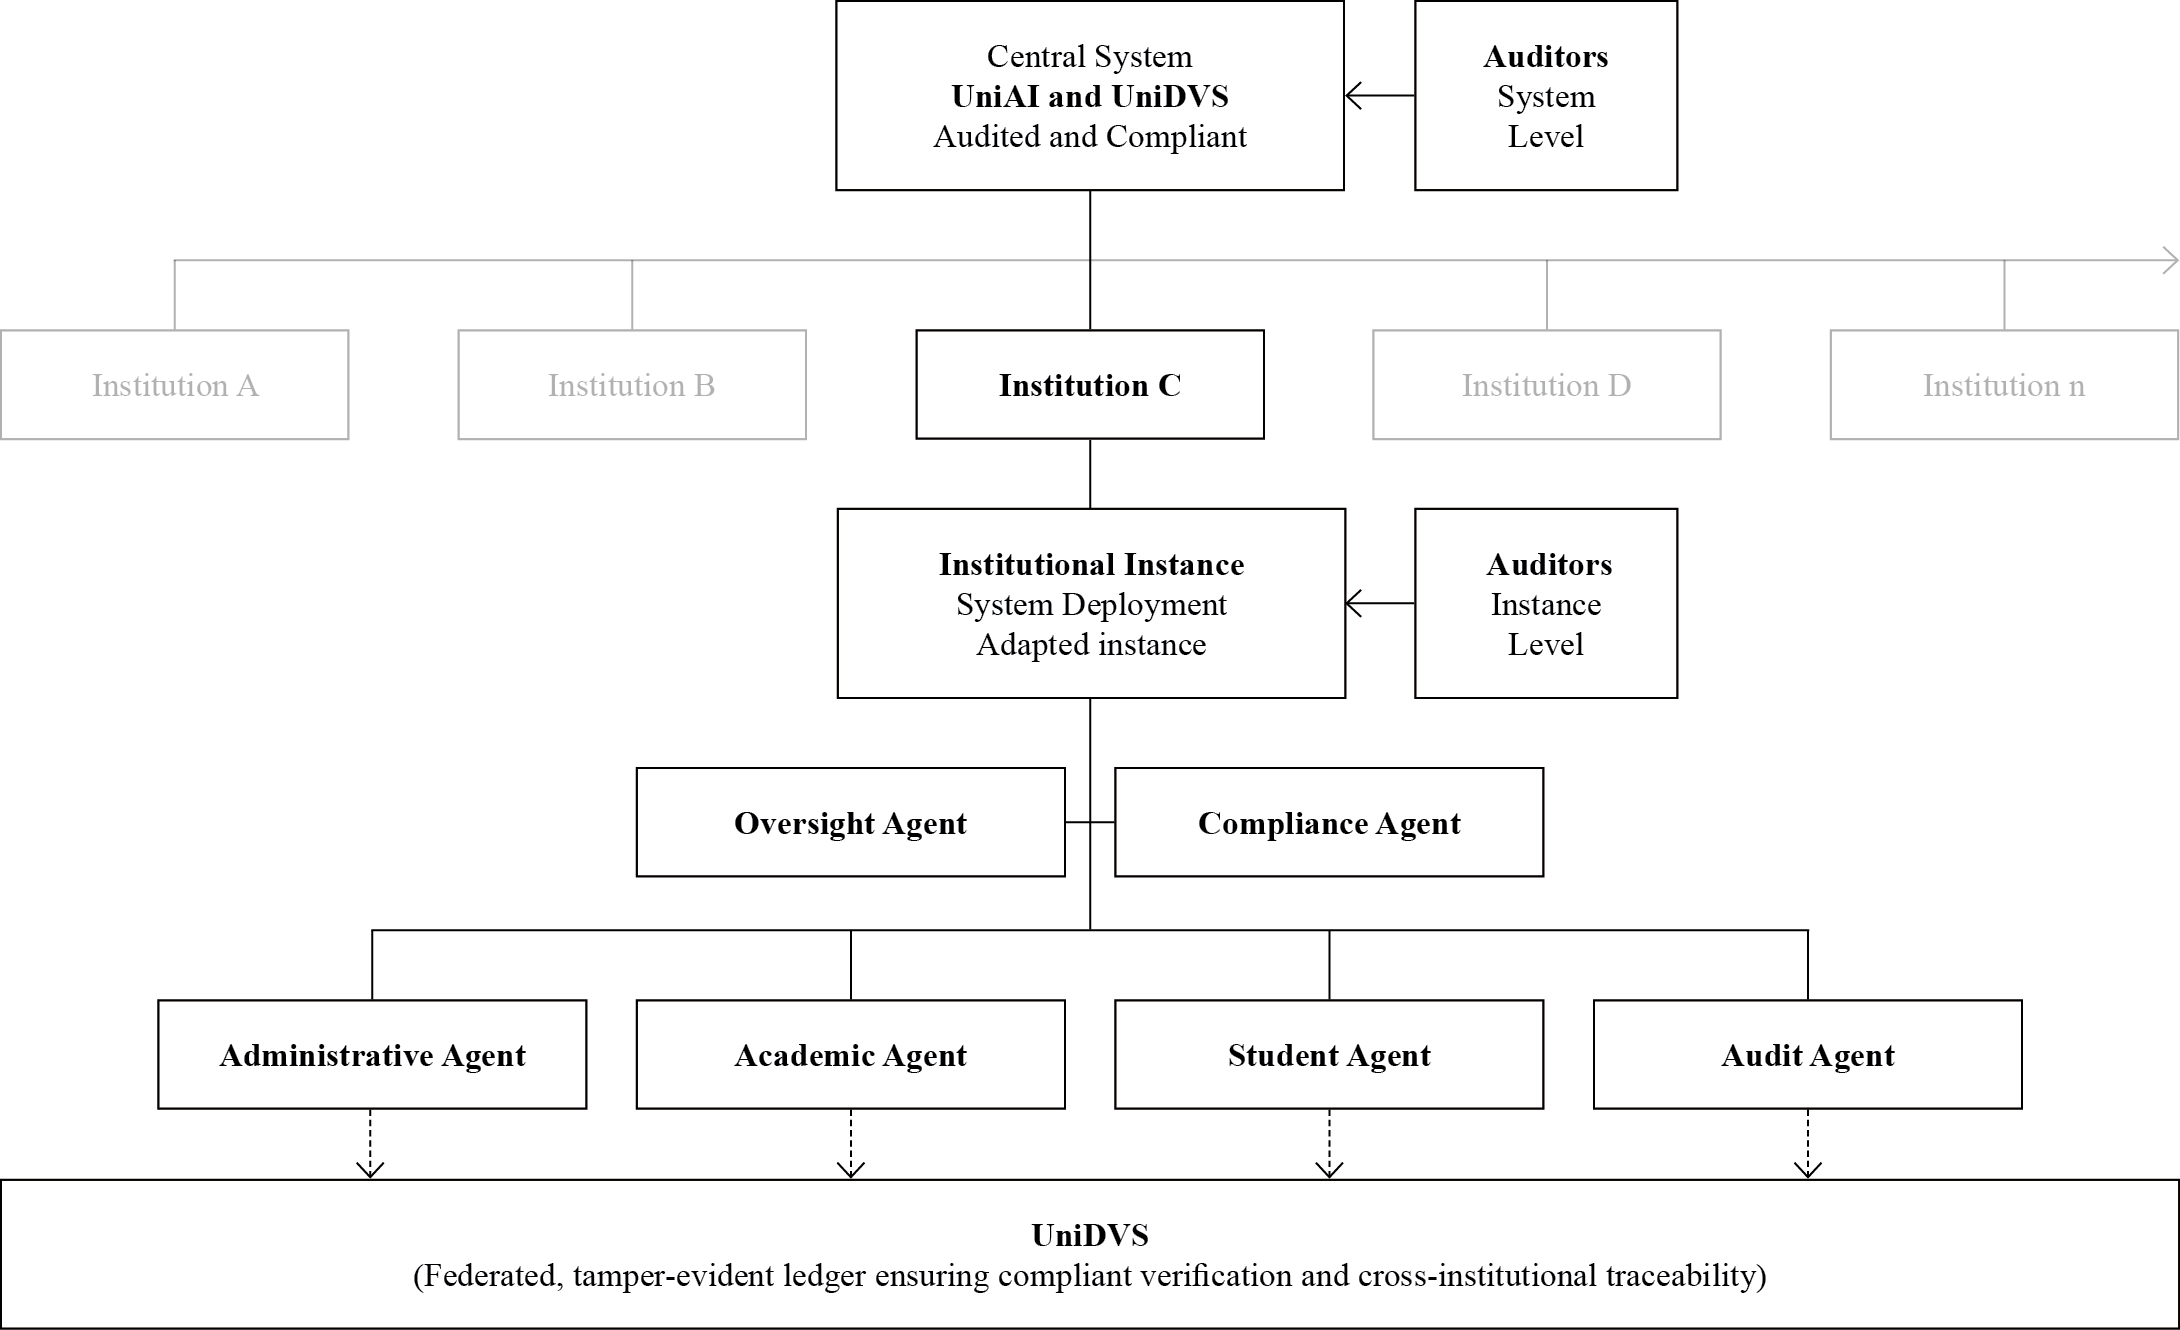
\includegraphics[width=\textwidth]{3-assets/1-User/DrWalterKurz_UniAI-2.png}
  \caption{Agent-based institutional architecture of UniAI and its linkage to the federated UniDVS layer.}
  \label{fig:UniAI-agents}
\end{figure}

The diagram separates the centralised core system from its institutional instances. Each participating institution operates a white-labelled deployment of UniAI, configured to local policies while remaining structurally aligned with the audited system core. Within each instance, agents are segmented by role. Administrative, academic, student, and audit agents perform domain-specific tasks. Oversight and compliance agents monitor rule adherence and ensure decisions remain within the constrained policy space $\Pi^\star$. All verifiable actions, including credential issuance, course registration, and institutional payments, are synchronised to UniDVS. This federated layer provides tamper-evident recordkeeping, legal admissibility, and audit access across jurisdictions. Auditors may inspect both the central system logic and the operational outputs of institutional deployments. The next subsection specifies each agent class and defines its operational function within the regulated execution environment.

\subsection{UniAI Agent Modelling by Stakeholder Role}

The UniAI subsystem is structured as a multi-agent architecture composed of role-specific agents, each aligned with the operational logic and normative expectations of defined institutional stakeholders. Unlike monolithic AI systems that optimise toward a single objective, UniAI maintains agent differentiation to reflect divergent stakeholder goals, procedural responsibilities, and authorisation levels within higher education institutions. Agent classes are derived from institutional role classifications, accreditation protocols, and accountability structures. Each agent operates within a defined mandate and generates outputs admissible under the system’s legal and organisational constraints. Administrative agents manage core institutional workflows. These include enrolment processing, timetable coordination, financial disbursement, and regulatory reporting. Their operation is governed by internal governance protocols and external audit requirements. Decision paths must remain transparent, traceable, and reversible within institutional audit cycles. These agents require high reliability, deterministic outputs, and controlled access to sensitive data, with execution rights over actions with contractual consequences. Academic agents operate within the domain of instructional staff. Responsibilities include curriculum management, assessment generation, grading support, and content validation. Their autonomy is restricted to predefined task sets and bounded by institutional quality assurance frameworks. Outputs must be interpretable, especially where decisions affect student progression, and must conform to disciplinary standards. Inference remains advisory unless formally validated through authorised human input. Student agents operate at the user-facing interface layer. They support course planning, workload estimation, credit tracking, and administrative navigation. Access is restricted to personal records and publicly available academic offerings. Outputs must be explainable and reversible. Agents may not trigger irreversible actions without authenticated human confirmation. Privacy requirements and user control take precedence, particularly in dynamic recommendation and procedural guidance. Audit agents constitute an independent verification layer. They monitor compliance with legal, procedural, and institutional constraints. Operating with read-only access to logs, credentials, and transactions, they produce compliance proofs and detect anomalies. Audit agents are epistemically conservative by design, prioritising evidentiary admissibility and traceable logic over autonomy. Their function is to validate both agent outputs and their consistency with the constraint set formalised in UniDVS. This role-specific agent architecture reflects the decentralised, interdependent structure of higher education institutions. Agents operate semi-autonomously within bounded mandates and are coordinated through the shared constraint logic and institutional objective defined in the preceding formalisation.

\subsubsection{Stakeholder-Specific Agent Objectives under Institutional Constraints}

The global objective of the UniAI and UniDVS architecture has been formalised as a regulation-compliant optimisation system (see Equation~\ref{eq:objective}). Within this framework, we now define the stakeholder-specific objectives of individual agents. The constraints expressed in Equation~\ref{eq:objective} are assumed to hold globally and remain structurally enforced. Agent-level formulations therefore omit explicit constraint clauses but operate entirely within the admissible policy space $\Pi^\star$. The system is not designed for full autonomous substitution. Instead, it functions as a structural support architecture. Although technical automation is feasible across many tasks, this trajectory is rejected by the authors. Institutional roles in administration, teaching, and auditing must be preserved. The argument is not limited to governance or oversight but includes macroeconomic stability. Removing employment from educational institutions in favour of AI efficiency would erode tax bases, reduce contributions to public insurance systems, and compromise the redistributive function of public sector employment. Educational systems contribute not only through knowledge provision but as stable, regionally embedded employers. UniAI is therefore conceived as an augmentation layer. Its function is to enhance procedural reliability, verifiability, and institutional integrity while preserving the human-institutional interface. Each UniAI agent class—administrative, academic, student, and audit—is modelled as an actor operating over the institutional state space $\mathcal{I}$, with role-specific objectives and scoped access. Agent actions are governed by utility functions $U_r$, indexed by role $r \in \{a, p, s, u\}$ for administration, professors, students, and auditors respectively. Let $\pi_r$ denote the policy associated with role $r$, parameterised by $\theta_r$.

\paragraph{Administrative Agents}

Administrative agents represent institutional operations such as enrolment management, fee processing, course scheduling, and academic record maintenance. Their function is to ensure procedural coherence, timely execution of workflows, and compliance with institutional statutes. UniAI agents in this category interact with sensitive personal and financial data, requiring accurate processing, strict access control, and verifiable audit trails. Their outputs directly affect institutional accountability and are often subject to both internal policies and external review. This agent class establishes the operational link to auditor agents, which draw on administrative output data to assess procedural validity and regulatory conformity. The architecture is designed to support both internal and external auditors—such as national accreditation bodies or financial supervisory authorities—by enabling controlled access to certified logs and compliance records. A human-in-the-loop mechanism remains embedded, ensuring that critical decisions, overrides, or institutional exceptions can only be validated through designated administrative oversight. The operational logic of administrative agents is derived as a sub-optimisation within the global system objective (cf.\ Equation~\ref{eq:objective}). These agents operate under role-specific policies $\pi_a$ parameterised by $\theta_a$, with utility function $U_a$ defined over a bounded administrative subspace $\mathcal{I}_a \subseteq \mathcal{I}$. Their role is to maximise procedural consistency, institutional reliability, and data integrity, while enforcing access constraints and auditability requirements. The corresponding optimisation problem is defined in Equation~\ref{eq:admin}:
\begin{align}
\label{eq:admin}
\max_{\pi_a} \quad & \mathbb{E}_{t \sim \mathcal{T}_a} \left[ U_a(t \mid \pi_a, \mathcal{I}_a) \right] \\
\text{subject to:} \quad
& \forall\, t \in \mathcal{T}_a: \nonumber \\
& \text{Access}(\pi_a(t)) \subseteq \mathcal{P}_a, \nonumber \\
& \text{Audit}(\pi_a(t)) \in \mathcal{V}_a \nonumber
\end{align}

where $\mathcal{T}_a$ is the set of administrative tasks (e.g.\ enrolment, record updating, payments), $\mathcal{P}_a$ defines the role-specific permission space for data access, and $\mathcal{V}_a$ denotes the verifiability requirements for audit integration. The equation defines the agent’s mandate to perform admissible actions within bounded institutional protocols while generating traceable, certifiable outcomes for downstream oversight.

\paragraph{Academic Agents}

Academic agents represent the role of faculty members within the institutional system. Their tasks include course design, instruction, grading, supervision of academic outputs, and contribution to curricular governance. UniAI agents in this role assist in workload management, grading standardisation, and curriculum alignment while preserving the autonomy of academic judgement. Outputs generated in this context must be explainable, reversible where necessary, and traceable for audit and appeal procedures. These agents interact with both UniDVS and human oversight channels to maintain the epistemic integrity of academic decisions. The system enforces strict boundaries between automated support and final academic authority, preserving faculty control over grading and certification. Professorial agents also participate in quality assurance processes and generate data for institutional reviews, requiring their policy outputs to be structurally aligned with institutional learning objectives and ESG-guided quality metrics. The objective of these agents is modelled as a constrained optimisation problem derived from the global system objective (see Equation~\ref{eq:academic}):
\begin{align}
\label{eq:academic}
\max_{\pi_p} \quad & \mathbb{E}_{t \sim \mathcal{T}_p} \left[ U_p(t \mid \pi_p, \mathcal{I}_p) \right] \\
\text{subject to:} \quad
& \forall\, t \in \mathcal{T}_p: \nonumber \\
& \text{Explainability}(\pi_p(t)) \geq \varepsilon_p, \nonumber \\
& \text{Traceability}(\pi_p(t)) \in \mathcal{V}_p, \quad \text{Authority}(\pi_p(t)) \subseteq \mathcal{A}_p \nonumber
\end{align}

Let $\mathcal{T}_p$ denote the task space of academic agents, encompassing actions such as grading, supervision, and curricular contributions. The policy $\pi_p$ maps academic tasks to decisions, parameterised by role-specific model parameters. The institutional subspace $\mathcal{I}_p$ encodes the state variables relevant to academic processes, including course structures, student submissions, and assessment protocols. The utility function $U_p$ quantifies the effectiveness and institutional validity of academic actions under the current policy. The constraints enforce minimum explainability of outputs (e.g.\ score justifications), traceability within the verification infrastructure $\mathcal{V}_p$, and alignment with permissible academic authority actions $\mathcal{A}_p$. $\varepsilon_p$ defines the institutional lower bound for explainability thresholds, ensuring that automated outputs can be subject to human review and appeal.

\paragraph{Student Agents}

Student agents represent learner interactions with institutional services, including course enrolment, assignment submission, progress monitoring, and feedback integration. UniAI supports these agents through personalised interfaces, adaptive recommendation mechanisms, and access to verifiable credential records. The agent policy operates within bounded permissions, ensuring that all interactions are valid, non-manipulable, and fully traceable. Importantly, student agents are designed not merely as passive recipients of institutional output but as active nodes within the verification infrastructure. Their inputs serve as verifiable events in audit chains, and their engagement patterns influence adaptive resource allocation, feedback cycles, and equity analysis. The objective function governing student agents is formally defined in Equation~\ref{eq:student}, which specifies their admissible behaviour within institutional and verification contexts.
\begin{align}
\label{eq:student}
\max_{\pi_s} \quad & \mathbb{E}_{t \sim \mathcal{T}_s} \left[ U_s(t \mid \pi_s, \mathcal{I}_s) \right] \\
\text{subject to:} \quad
& \forall\, t \in \mathcal{T}_s: \nonumber \\
& \pi_s(t) \in \mathcal{P}_s, \nonumber \\
& \gamma(t) \in \mathcal{V}_s, \nonumber \\
& \phi(t) \geq \varepsilon_s \nonumber
\end{align}

Let $\mathcal{T}_s$ denote the task space of student agents, encompassing actions such as enrolment, submission, query, and credential access. The policy $\pi_s$ maps student tasks to executable decisions, constrained by the set of permitted interactions $\mathcal{P}_s$. The institutional subspace $\mathcal{I}_s$ comprises student-specific state variables such as enrolment status, academic progression, and credential portfolios. $\gamma(t)$ encodes the verifiability of the student interaction under UniDVS, and $\phi(t)$ denotes the interpretability score of system responses, constrained to exceed threshold $\varepsilon_s$ to ensure transparency. $U_s$ is the utility function measuring procedural coherence, accessibility, and learning progression quality under policy $\pi_s$.

\paragraph{Auditor Agents}

Auditor agents operate at the meta-institutional layer of UniAI and serve to validate the procedural and regulatory correctness of operations executed across the system. Unlike agents focused on service delivery or stakeholder interaction, auditors function retrospectively, applying normative filters to verify that recorded actions adhere to institutional policy, jurisdictional law, and auditability requirements. These agents interact with academic, administrative, and financial outputs, assessing their legitimacy, rule compliance, and exception status. Auditor agents may act on behalf of internal governance bodies or external regulators and accreditors. Their policy logic is not geared toward optimisation but toward consistency, traceability, and evidentiary alignment.
A mandatory human-in-the-loop protocol is enforced to ensure that legal conclusions, compliance verdicts, and audit certifications remain under accountable human authority. The agent policy for this role is defined as a constrained optimisation problem in Equation~\ref{eq:auditor}, capturing the logic of verifiable assessment under procedural and human oversight constraints:
\begin{align}
\label{eq:auditor}
\max_{\pi_u} \quad & \mathbb{E}_{t \sim \mathcal{T}_u} \left[ U_u(t \mid \pi_u, \mathcal{I}_u) \right] \\
\text{subject to:} \quad
& \forall\, t \in \mathcal{T}_u: \nonumber \\
& \text{Trace}(\pi_u(t)) \in \mathcal{H}_u, \nonumber \\
& \text{Justify}(\pi_u(t)) \in \mathcal{E}_u, \quad \text{Approval}(\pi_u(t)) \in \mathcal{H}_{\text{human}} \nonumber
\end{align}

Here, $\pi_u$ is the auditor agent policy, parameterised by $\theta_u$, over the task distribution $\mathcal{T}_u$ and institutional state space $\mathcal{I}_u$. The utility function $U_u$ encodes audit-relevant objectives such as procedural completeness, regulatory adherence, and anomaly detection. The constraint set includes: $\text{Trace}(\pi_u(t)) \in \mathcal{H}_u$, ensuring all agent actions are reconstructable via cryptographic or procedural logs; $\text{Justify}(\pi_u(t)) \in \mathcal{E}_u$, requiring logical or evidentiary grounds for compliance verdicts; and $\text{Approval}(\pi_u(t)) \in \mathcal{H}_{\text{human}}$, mandating that critical audit outcomes are subject to human authorisation.

\subsubsection{System Coordination, Auditability, and Governance Integration}

The deployment of UniAI and UniDVS across institutional environments requires a coordinated operational framework that ensures coherent interaction among autonomous agents, traceable decision-making, and enforceable oversight. This subsection formalises the systemic mechanisms by which agent-level objectives, as defined in the previous section, are orchestrated within a verifiable and governable infrastructure.

Coordination mechanisms ensure consistency across agent outputs and resolve inter-role dependencies. For example, academic assessments processed by UniAI professors must synchronise with administrative agents for credential issuance and be made accessible to audit agents for compliance verification. This necessitates formal checkpointing, shared institutional state representations, and asynchronous task resolution protocols.

Auditability is enforced through cryptographically verifiable logs, role-specific access registries, and tamper-evident data trails. Each action performed by an UniAI agent is recorded within a decentralised ledger maintained by UniDVS, ensuring that regulatory bodies, accreditation authorities, and internal governance boards retain the capacity to reconstruct decision pathways ex post.

Governance integration encodes institutional authority structures directly into the operational logic of UniAI. Human oversight is not a fallback mechanism but a formalised execution layer. Administrative override privileges, audit inspection rights, and dispute resolution processes are explicitly specified and enforced within the coordination architecture. Versioning of system updates—including model adjustments and policy retraining—is governed by institutional protocols and subject to supervisory control. The coordination logic governing multi-agent interaction across institutional roles is formalised in Equation~\ref{eq:coordination}, defining the collective optimisation function and its enforceable constraints:
\begin{align}
\label{eq:coordination}
\max_{\{\pi_r\}_{r \in \{a, p, s, u\}}} \quad & \mathbb{E}_{(r, t) \sim \mathcal{D}} \left[ U_r(t \mid \pi_r, \mathcal{I}) \right] \\
\text{subject to:} \quad
& \text{(C1)} \quad \text{Consistency}(\pi_r(t), \pi_{r'}(t')) \in \mathcal{C}_{\text{sync}} \quad \forall\, (r, r') \in \mathcal{R}^2, \nonumber \\
& \text{(C2)} \quad \text{Trace}(\pi_r(t)) \in \mathcal{L}_{\text{ledger}}, \nonumber \\
& \text{(C3)} \quad \text{Governance}(\pi_r) \subseteq \mathcal{G}_{\text{institutional}}, \nonumber \\
& \text{(C4)} \quad \text{AuditAccess}(\pi_r(t)) \in \mathcal{A}_{\text{auditors}} \nonumber
\end{align}

$\pi_r$ denotes the policy for agent role $r \in \{a, p, s, u\}$ acting on institutional tasks $t \in \mathcal{T}_r$ drawn from the global task distribution $\mathcal{D}$. $\mathcal{C}_{\text{sync}}$ defines admissible synchronisation constraints across agent interactions. $\mathcal{L}_{\text{ledger}}$ is the set of valid audit log entries maintained by UniDVS. $\mathcal{G}_{\text{institutional}}$ encodes institutional approval and override structures. $\mathcal{A}_{\text{auditors}}$ defines the access scope for internal and external audit agents. The optimisation governs coordinated execution, traceability, and compliance across all UniAI components.

\subsection{Dual-Layer UniDVS Architecture}

UniDVS is not conceived as a centralised registry but as a decentralised verification ecosystem jointly maintained by accredited institutions and regulatory authorities. This structure reflects the federated model of higher education governance and ensures that no single vendor, institution, or administrative actor exercises unilateral control over the verification layer. Verifiability results from distributed consensus and cryptographic commitment across independent, interoperable nodes.

Each participating node operates a validator instance responsible for transaction verification, certification attestation, and ledger synchronisation. Validator nodes are operated by universities, quality assurance bodies, credential recognition authorities, and regulatory agencies in finance and data protection. The inclusion of regulatory actors ensures that technical verification aligns with legal admissibility and provides direct read-access to certified records for supervisory inspection and audit.

To accommodate institutional heterogeneity and asynchronous propagation, the system implements a directed acyclic graph (DAG) consensus mechanism instead of a linear blockchain. Unlike blockchains, DAGs permit concurrent transaction validation without requiring global ordering. This reduces latency, increases scalability, and enables parallel commitment of verified outputs, including diploma issuance, assessment records, and audit trails, without introducing central bottlenecks. Each transaction is cryptographically linked to its predecessors, ensuring traceability and non-repudiation while avoiding the throughput constraints of sequential consensus architectures.

We propose to implement UniDVS as a two-layer infrastructure. Layer~1 serves as the primary ledger for regulated institutional outputs, including the transfer of stablecoins, issuance of ECTS tokens, and registration of educational transactions with financial or legal consequences. This layer may operate under controlled economic incentives and supports activities that require formal auditability and monetary traceability.

Layer~2 functions as a high-throughput, non-incentivised submission environment for procedural and technical interactions that do not involve value transfer. This includes credential attestations, course structure updates, institutional metadata submissions, and system-generated logs. Layer~2 is optimised for low-latency, cost-free operation, reflecting the operational role of academic and administrative agents acting within their institutional mandates.

To preserve evidentiary integrity and ensure external verifiability, Layer~2 periodically anchors aggregated state commitments into Layer~1. Anchoring methods may include Merkle root submissions, hash commitments, or recursive proofs that represent the institutional verification state over defined intervals.

The formal objective of the UniDVS architecture is expressed as a distributed optimisation problem in Equation~\ref{eq:dag}. It defines the admissible policy space for graph-based verification and institutionally coordinated state propagation.
\begin{align}
\label{eq:dag}
\max_{\pi_{\text{dvs}}} \quad & \mathbb{E}_{e \sim \mathcal{E}} \left[ U_{\text{dvs}}(e \mid G, \mathcal{N}) \right] \\
\text{subject to:} \quad
& \forall\, e \in \mathcal{E}: \quad \text{Sig}(e) \in \mathcal{K}_n, \quad \text{Parent}(e) \subseteq G, \nonumber \\
& \forall\, n \in \mathcal{N}: \quad \text{Role}(n) \in \mathcal{R}_{\text{edu}} \cup \mathcal{R}_{\text{reg}}, \quad \text{Consistency}(G) = \text{True}, \nonumber \\
& \text{Finality}(e) \Rightarrow \text{Auditability}(e) = \text{True} \nonumber
\end{align}

Here, $\pi_{\text{dvs}}$ denotes the system policy governing validation and propagation of verification events $e$ within the graph $G$, maintained by institutional nodes $\mathcal{N}$. Each event must be signed with a valid institutional key from $\mathcal{K}_n$ and reference valid predecessors via $\text{Parent}(e)$. Node roles are classified under $\mathcal{R}_{\text{edu}}$ for educational entities and $\mathcal{R}_{\text{reg}}$ for supervisory authorities. $\text{Consistency}(G)$ ensures the graph remains acyclic and coherent. $\text{Finality}(e)$ marks transaction commitment, requiring that its audit trail remains intact and externally verifiable.

Interaction with UniDVS is structured through role-specific verification channels $\mathcal{V}_r$, which define submission, querying, and contestation rights for each agent type $r \in \{a, p, s, u\}$. These interactions are subject to strict protocol rules that determine admissibility for ledger inclusion. The formal rule for conditional commitment of actions to the UniDVS ledger is defined in Equation~\ref{eq:UniDVS}:
\begin{align}
\label{eq:UniDVS}
\forall\, r \in \{a, p, s, u\}, \, \forall\, t \in \mathcal{T}_r: \quad
\text{Submit}(\pi_r(t)) \rightarrow
\begin{cases}
\text{Commit}(\pi_r(t)) \in \mathcal{L}_{\text{DVS}}, & \text{if } \pi_r(t) \models \mathcal{C}_{\text{DVS}} \\
\bot, & \text{otherwise}
\end{cases}
\end{align}

Here, $\text{Submit}(\pi_r(t))$ denotes the agent’s intent to register an action $t$ under policy $\pi_r$. The verification logic $\mathcal{C}_{\text{DVS}}$ includes institutional approval status, cryptographic signature validity, time-window conditions, and inter-agent coherence checks. Once verified, the action is committed to $\mathcal{L}_{\text{DVS}}$, the decentralised institutional ledger, where it becomes publicly auditable and synchronised across all participating institutions.

UniAI agents must be capable of distinguishing between Layer~1 and Layer~2 transaction domains. Layer~1 is reserved for actions with formal regulatory, financial, or cross-institutional consequences, including stablecoin transfers, ECTS token issuance, and notarised contract registration. Layer~2 supports procedural, low-latency submissions such as metadata updates, non-monetary attestations, and internal audit traces. Submission logic is governed by a taxonomy of smart contract classes. Contracts requiring legal finality, fiscal auditability, or external anchoring are classified as $\mathcal{S}_1$ and routed to Layer~1. Contracts used for procedural synchronisation, internal recordkeeping, or non-monetary agent coordination are classified as $\mathcal{S}_2$ and executed on Layer~2. Combined contract structures, denoted $\mathcal{S}_{1+2}$, may span both layers: they initiate in Layer~2 and commit hash-verified final states to Layer~1. UniAI agents must resolve the correct layer designation at submission time based on encoded policy type, agent role, institutional scope, and downstream dependency conditions. To ensure evidentiary consistency and correct execution routing, agents must dynamically resolve the target layer for each contract at runtime. Table~\ref{tab:smartcontracttaxonomy} defines the classification scheme used to assign smart contracts according to their regulatory function, execution scope, and anchoring requirement. This structure supports layered verifiability, procedural efficiency, and compliance integrity~\cite{eu2023mica, eu2014mifid2, eu2016gdpr}.
\begin{table*}[ht]
\centering
\caption{Smart contract taxonomy for AI-based layer assignment}
\label{tab:smartcontracttaxonomy}
\small
\begin{tabularx}{\textwidth}{@{}X L{4.8cm} L{5.2cm} L{2.2cm}@{}}
\toprule
\textbf{Contract Class} & \textbf{Typical Functions} & \textbf{Submission Criteria} & \textbf{Assigned Layer} \\
\midrule
\textbf{S\textsubscript{1}} (Regulatory Finality) & Stablecoin transfers, ECTS issuance, institutional payments, notarised agreements, external obligations & Requires auditability, triggers financial/legal obligations, needs cross-institutional traceability & Layer 1 \\
\textbf{S\textsubscript{2}} (Technical Attestation) & Credential uploads, course structure changes, system status logs, user role updates & Internal institutional provenance, low financial impact, procedural transparency only & Layer 2 \\
\textbf{S\textsubscript{3}} (Hybrid Synchronisation) & Inter-agent delegation records, regulatory notices, inter-consortium state events & Dual requirements for immutability and speed, needs anchoring to L1 & Layer 2 + Anchor to Layer 1 \\
\bottomrule
\end{tabularx}
\end{table*}

Tasks initiated by institutional stakeholders often encapsulate multiple minting operations spanning distinct regulatory and procedural domains. UniAI agents must decompose each high-level task specification into discrete minting actions, with each action aligned to its corresponding compliance constraints. This requires classifying intended outputs using the smart contract taxonomy defined in Table~\ref{tab:smartcontracttaxonomy}, selecting the appropriate contract template, and parameterising it with task-specific attributes such as issuer credentials, validity period, audit scope, and financial linkage.

Each minting action must be executed in the appropriate system layer: Layer~1 for legally binding artefacts, Layer~2 for procedural submissions, or both where cryptographic anchoring is required. Logical consistency must be preserved across all minted outputs. Agents must ensure that auditability, finality, and verifiability conditions are satisfied without redundancy, omission, or cross-layer misclassification.

The minting logic executed by UniAI agents can be formalised as a constrained optimisation problem, shown in Equation~\ref{eq:minting}. This formulation expresses the agent’s responsibility to infer, classify, and execute a valid sequence of minting operations from a structured task specification, subject to semantic and regulatory constraints.
\begin{align}
\label{eq:minting}
\max_{\mu} \quad & \sum_{i=1}^{n} \delta(m_i, \tau_i) \cdot V(m_i) \\
\text{subject to:} \quad
& \forall\, m_i \in \mathcal{M}: \quad \text{Class}(m_i) = \text{Tax}(\tau_i), \nonumber \\
& \text{Layer}(m_i) = \lambda(\text{Class}(m_i)), \quad \text{Template}(m_i) \models \text{Req}(\tau_i), \nonumber \\
& \text{Finality}(m_i) \Rightarrow \text{Verifiability}(m_i) = \text{True}, \quad \text{Mint}(m_i) \Rightarrow \text{Submit}(m_i) \in \mathcal{L}_{\text{DVS}} \nonumber
\end{align}

Here, $\mu$ denotes the agent policy for minting, and $\mathcal{M} = \{m_1, \dots, m_n\}$ the set of mintable artefacts derived from the stakeholder task. Each artefact $m_i$ is evaluated against a corresponding task component $\tau_i$, where $\delta(m_i, \tau_i)$ expresses semantic alignment and $V(m_i)$ denotes the compliance or operational value of the artefact. The function $\text{Class}(\cdot)$ assigns a contract class based on the smart contract taxonomy $\text{Tax}(\cdot)$, and $\lambda(\cdot)$ maps this class to the required system layer. The selected template $\text{Template}(m_i)$ must fulfil the requirements $\text{Req}(\tau_i)$ encoded in the task specification. Finality enforces verifiability, and successful minting implies valid submission to the decentralised verification ledger $\mathcal{L}_{\text{DVS}}$.

At Layer~1 of the UniAI architecture, the federated compliance environment operated and supervised by accredited consortia, we propose the implementation of a reference system to support classification resolution in ambiguous cases. UniAI agents are expected to autonomously infer valid minting pathways and select the appropriate contract class and system layer. However, atypical or previously unobserved input structures may exceed the agent’s generalisation capacity. To support decision-making in such cases, we include a curated case reference list that maps representative institutional tasks to validated contract classifications. This retrieval mechanism improves robustness in edge cases and aligns agent execution with institutional precedent.

In addition to historical inference support, we propose that participating institutions jointly maintain a normative list of Layer~1 and Layer~2 contract categories. This list defines which submissions incur transaction costs and which remain exempt. It serves as a governance mechanism that allows institutional actors to steer operational incentives while preserving accessibility for core academic functions. Submissions related to monetary value transfer or formal rights issuance may be subject to fee-based validation, whereas procedural interactions—such as course structure updates or internal attestations—should remain free of charge. The classification list and its underlying contract taxonomy are subject to periodic review by the governing consortium, ensuring responsiveness to regulatory, pedagogical, and operational developments.

To formalise the contract classification logic applied by UniAI agents at Layer~1, we define an equation that integrates case-based inference, normative rules, and model-based reasoning into the agent's layer selection process. This structure ensures that each minting task is accurately mapped to the appropriate system layer, as shown in Equation~\ref{eq:layerclassification}:
\begin{align}
\label{eq:layerclassification}
\text{Layer}(\tau_i) =
\begin{cases}
\text{Lookup}(\tau_i, \mathcal{C}) & \text{if } \tau_i \in \text{Dom}(\mathcal{C}) \\
\text{GovernanceRule}(\tau_i, \mathcal{G}) & \text{if } \tau_i \in \text{Dom}(\mathcal{G}) \\
\text{InferLayer}(\tau_i, \theta_r) & \text{otherwise}
\end{cases}
\end{align}

Here, $\tau_i$ denotes the $i$-th minting task submitted by an agent. The function $\text{Lookup}(\tau_i, \mathcal{C})$ performs case-based retrieval from the curated classification list $\mathcal{C}$, which maps previously verified task types to their corresponding execution layers. If no historical match is found, the agent queries $\text{GovernanceRule}(\tau_i, \mathcal{G})$, where $\mathcal{G}$ defines the consortium-maintained classification logic for distinguishing fee-based from non-fee-based submissions. If both mechanisms fail to resolve the classification, the agent defaults to $\text{InferLayer}(\tau_i, \theta_r)$, which applies its learned policy $\theta_r$ to determine the appropriate contract layer. This formalism constrains agent behaviour within a bounded decision space that integrates institutional precedent, governance policy, and model-based generalisation.

\subsection{Tokenised Assets and Stablecoin Integration for Institutional Operations}

Within the UniDVS framework, tokenised assets are implemented to support institutional documentation, accounting, and credit transfer across jurisdictions. These assets comprise two classes: a unified, jurisdiction-approved institutional stablecoin, and verifiable ECTS tokens representing academic achievements. Both operate within the same technical infrastructure but fulfil distinct regulatory and operational functions.

The institutional stablecoin is a single, regulatory-approved digital asset registered across participating jurisdictions, including Switzerland and the European Union. It qualifies as a financial instrument and complies with applicable instruments such as the Swiss Financial Market Infrastructure Act (FMIA) \cite{ch2016fima}, Financial Services Act (FinSA) \cite{ch2018finsa}, and Anti-Money Laundering Act (AMLA) \cite{ch2021amla}, as well as EU-level frameworks including the Markets in Crypto-Assets Regulation (MiCA) \cite{eu2023mica}, the Markets in Financial Instruments Directive (MiFID II) \cite{eu2014mifid2}, the Second Electronic Money Directive (EMD2) \cite{eu2009emd2}, and the 6th Anti-Money Laundering Directive (AMLD) \cite{eu2018amld6}. Supervision is exercised by FINMA \cite{finma2024}, ESMA \cite{esma2024}, and national competent authorities \cite{bafin2024,fma2024}. The stablecoin is backed by institutional reserves and functions as a programmable, tamper-proof medium for internal disbursements, tuition payments, and inter-institutional settlements. Its use ensures financial compliance, auditability, and traceable value flows across higher education networks.

ECTS tokens represent formalised academic credits aligned with the European Credit Transfer and Accumulation System (ECTS) \cite{ec2015ects}, the European Qualifications Framework (EQF) \cite{ec2017eqf}, and the Bologna Process \cite{ehea2020bologna}. Although not classified as financial instruments, they carry legal significance within qualification frameworks and student financing schemes. ECTS tokens are issued by accredited institutions, with compliance and integrity monitored through UniDVS by national quality assurance bodies and recognition authorities, including ENQA \cite{enqa2015esg}, AAQ \cite{aaq2024}, the German Accreditation Council \cite{germanaccreditation2022}, NVAO \cite{nvao2023}, and ANECA \cite{aneca2023}. Each token is cryptographically verifiable, traceable, and immutable once recorded in the decentralised infrastructure.

\section{Discussion}

The proposed architecture demonstrates that legally operable, multi-agentic AI systems and decentralised verification infrastructures can be integrated into higher education without undermining institutional autonomy or regulatory compliance. Legal constraints are embedded directly into system logic, avoiding externalised compliance layers and enforcing admissibility, traceability, and auditability as structural properties. The separation of UniAI and UniDVS functions ensures that decision-making and verification remain modular yet interoperable, aligned with existing governance structures.

UniAI operates across three structural layers: centralised system governance, institutional deployment, and independent oversight. This separation preserves a functional boundary between algorithmic automation and institutional authority. Agents are role-specific, constraint-bound, and auditable across jurisdictional and organisational contexts. Their actions are verifiable and legally admissible through a federated infrastructure grounded in regulatory frameworks.

UniDVS is structured as a two-layer system that supports institutional and cross-institutional verification. Layer~2 provides the primary operational environment for institutional processes. It records verifiable actions such as credential issuance, enrolment confirmations, and financial disbursements within a tamper-evident ledger maintained by participating institutions. Layer~1 serves as the anchoring layer for evidentiary integrity. It registers aggregated state proofs, such as Merkle roots or recursive hashes, over defined intervals to ensure global verifiability. Both layers are governed by a federated consortium, avoiding external dependencies and maintaining regulatory alignment.

Layer~2 of UniDVS is not profit-oriented. It is implemented as a non-incentivised infrastructure with structurally minimised transaction fees. Selected operations, including course attestations and credential submissions, may be executed without cost. This design ensures that institutional transactions remain aligned with public mandates and free from external fee regimes. In contrast, Layer~1 may be operated under a separate economic logic, including incentivised participation, provided that it remains under consortium governance and meets the evidentiary and supervisory requirements defined by the network. To ensure verifiability beyond the federated Layer~2 environment, UniDVS periodically anchors institutional state commitments to Layer~1. This anchoring guarantees traceability and evidentiary immutability without exposing internal institutional processes to market-based transaction costs or external dependency.

Technical scalability and regulatory interoperability have been addressed through formal modelling; however, empirical validation remains essential. Future work must include controlled deployments, stakeholder testing, and procedural stress scenarios to assess institutional trust, legal defensibility, and system resilience. While the model is jurisdiction-specific to Switzerland and the EU, it offers a transferable blueprint for comparable legal systems.

The architectural separation between utility-maximising agents and decentralised verifiability infrastructure introduces a normative constraint system that is resistant to unilateral override and open to institutional audit. The proposed token infrastructure, comprising a jurisdiction-approved stablecoin and verifiable ECTS-denominated credits, maintains financial precision and academic integrity in digital environments. The model demonstrates that AI-supported educational infrastructure can remain governable, auditable, and aligned with public-sector obligations without reducing education to a procedural service.

\section{Limitations and Further Research}

This framework defines a regulation-aligned architecture for AI-supported institutional operations and distributed verification in higher education. Its practical implementation remains subject to several limitations that require further investigation across 1technical, legal, and institutional domains.

Empirical research must evaluate system performance under realistic operating conditions, including enrolment workflows, credit transfer across jurisdictions, and audit procedures. Limitations include the current lack of tested response mechanisms for failure cases such as credential disputes, asynchronous ledger propagation, or conflicting jurisdictional claims.

The interaction between human oversight and autonomous UniAI agents has not yet been formalised in operational detail. This includes override capabilities, escalation protocols, and traceable decision chains that meet evidentiary standards under regulatory inspection. These gaps pose risks to procedural accountability and legal admissibility in contested decisions.

The governance structure of the decentralised UniDVS system also requires further specification. Open questions remain regarding validator eligibility, institutional legitimacy, and fault tolerance across the federated network. Without a clearly defined governance model, the infrastructure risks misalignment with accreditation frameworks and supervisory authority requirements.

Finally, the legal and monetary status of digital instruments issued through the system remains unresolved. The stablecoin component requires coordinated approval across financial regulators. ECTS-aligned tokens must be recognised under national and cross-border frameworks for credit accumulation and qualification recognition. These instruments cannot be operationalised without structured legal validation, formal regulatory testing, and controlled deployment within accredited institutional environments.

\bigskip

\bigskip

\printbibliography

\swDeclarationsPage

\end{document}
